\section{Methods} \label{sec:methods}

This section details the algorithm and implementation design used in this work.
After briefly recounting the core mechanics of hereditary stratigraphy methods for phylogenetic tracking, we motivate and describe new lightweight ``surface'' data structures used to annotate agent genomes in this work.
Then, we describe the asynchronous compute-communicate implementation strategy behind the testbed WSE-oriented island-based genetic algorithm used for validation and benchmarking experiments.

\begin{figure*}
  \centering
  \begin{subfigure}[t]{0.43\linewidth}
    \centering
  \includegraphics[width=\linewidth]{binder-wse-sketches/tex-access-proposal/img/runtime-posthoc-schematic}
    \caption{%
    Proposed agent-based evolutionary simulation and observation framework, using HStrat markers to estimate phylogenetic history, thereby, infer evolutionary dynamics.
    }
    \label{fig:runtime-posthoc-schematic}
  \end{subfigure}
  \hspace{0.07\linewidth}
  \begin{subfigure}[t]{0.43\linewidth}
    \centering
  \includegraphics[width=\linewidth]{binder-wse-sketches/tex-access-proposal/img/async-ga-schematic}
    \caption{Schematic overview of asynchronous island model evolutionary algorithm implementation.}
    \label{fig:async-ga-schematic}
  \end{subfigure}

\caption{%
\textbf{Summary of proposed experimental framework.}
Subfigure \ref{fig:runtime-posthoc-schematic} overviews proposed distributed simluation strategy.
Subfigure \ref{fig:async-ga-schematic} summarizes asynchronous population exchange strategy used to simulate evolving populations on Cerebras Wafer Scale Engine hardware.
}
\label{fig:schematic}

\end{figure*}


\subsection{Distributed Phylogenetic Tracking}

Natural history of biological life operates under no extrinsic provision for interprable record-keeping, yet efforts to study it have proved immensely fruitful.
This fact bodes well that scaled-up simulation studies can succeed a platform for rich hypothesis-driven experiments despite potential sacrifices to aspects of observability currently enjoyed with centralized, storage-rich processing.
Indeed, observational and analytical strategies already developed to confront limitations in biological data can solve, or at least guide, work with massively distributed evolution simulations.

In biology, decoupled processes of mutational drift encodes ancestry information in DNA genomes.
Prooposed methods approach analysis of evolutionary operates analogously, with ancestry information contained within genomes themselves rather than in any external tracking mechanism.
Phylogenetic history can then be estimated after-the-fact, as depicted in Figure \ref{fig:runtime-posthoc-schematic}.
This ensures low runtime communication overhead, as well as near total resiliency to germane modes of data loss (e.g., dropped messages, hardware crash-out).

Recent work introducing \textit{hereditary stratigraphy} (hstrat) methodology has explored how best to organize genetic material to maximize reconstruction quality and minimize memory footprint \citep{moreno2022hstrat, moreno2022hereditary}.
hstrat material can be bundled to agent genomes in a manner akin to non-coding DNA, entirely neutral with respect to agent traits and fitness.

The hereditary stratigraphy algorithm associates each generation along individual lineages with an identifying ``fingerprint'' value, referred to as a differentia.
On birth, offspring generate a new differentia value and append it to an inherited chronological record of differentia values, each corresponding to a generation along that lineage.
Under this scheme, mismatching differentia can be used to delimit the extent of common ancestry.
This semantic streamlines \textit{post hoc} phylogenetic reconstructio to a simple trie-building procedure
\citep{moreno2024analysis}.

To save space, differentia may be pruned away.
However, care must be taken to ensure retention of checkpoint generations that maximize coverage across evolutionary history.
Downsizing bits per differentia can also save memory space.
For instance, single-bit differentia occupy $32\times$ less memory than full-word differentia.
Such space savings can be invested to increase the quantity of differentia retained, improving the density of records' coverage across elapsed generations.
However, it comes at the cost of increased probability for spurious differentia value collisions, which can make two lineages appear more closely related than they actually are.
We anticipate that most use cases will call for differentia sized on the order of a single bit or a byte.
Indeed, single-bit differentia have been shown to yield good quality phylogenies using only 96 bits per genome \citep{TODOOTHERPAPER}.

Small differentia size intensifies need for a lean data structure to back differentia record management.
In particular, shrinking differentia to a single bit absurdifies accompanying each with a generational timestamp.
To safely drop timestamps, though, we must have means to recalculate them on demand.
As such, all described algorithms include means to deduce timestamps of retained differentia solely from their storage index and the count of the record's elapsed generations.

As a final elaboration, design of hstrat annotations must also consider how available storage space should be allocated across the span of history.
In one possible stategy, retained time points would be distributed evenly across history.
In another, more-recent time points would be preferred.
We term these as ``steady'' and ``tilted'' policies, respectively \citep{THEPAPERWHERETHETERMSAREFROMTODO}.
Note that prior hereditary stratigraphy work refers to them instead as ``depth-proportional'' and ``recency-proportional resolution.''
Comparisons of reconstruction quality have shown that tilted policy gives higher quality reconstructions from the same amount of reconsttruction space in most --- but not all --- circumstances \citep{oTHERPAPERTODO}.
This pattern follows an intuition to prefer high absolute precision is more useful to resolving recent events than more ancient ones.
In practice, it may be desirable to use a hybrid approach that allocates half of annotation space to each strategy \citep{oTHERPAPERTODO}.
Figure \ref{fig:surf-algorithms} includes retention drip plots that contrast behavior of steady and tilted algorithms.

\subsection{Surface-based Hereditary Stratigraphy Algorithms}

% Although designed with efficiency in mind, existing ``column''-based  have several properties that make them a poor fit with a resource-constrained environment like the the Cerebras WSE:
At the outset of this project, several problematic aspects of porting existing hereditary stratigraphy algorithms to the WSE became apparent.
Issues stemmed, in part, from a fundamental feature of these algorithms: organization of retained strata in contiguous, sorted order.
Forthwith, we refer to algorithms following this convention as ``column''-based.
The columnn design, and attendant implementation details, impose various drawbacks:
\begin{itemize}
\item \textbf{wated space}: an annotation size cap can be guaranteed, but a percentage of available space typically goes unused;
\item \textbf{high-level feature dependencies:} in places, existing column code usse complex data structures with dynamically allocated memory to perform operations like set subtraction,
\item \textbf{annotation size scaling:} slide-down procedures to maintain sorted order among differentia can take time linearly proportional to annotation size.
% \item \textbf{expensive operations:} in places, slow divide and modulo operations. heavy use
\end{itemize}

\begin{figure}
  \centering
  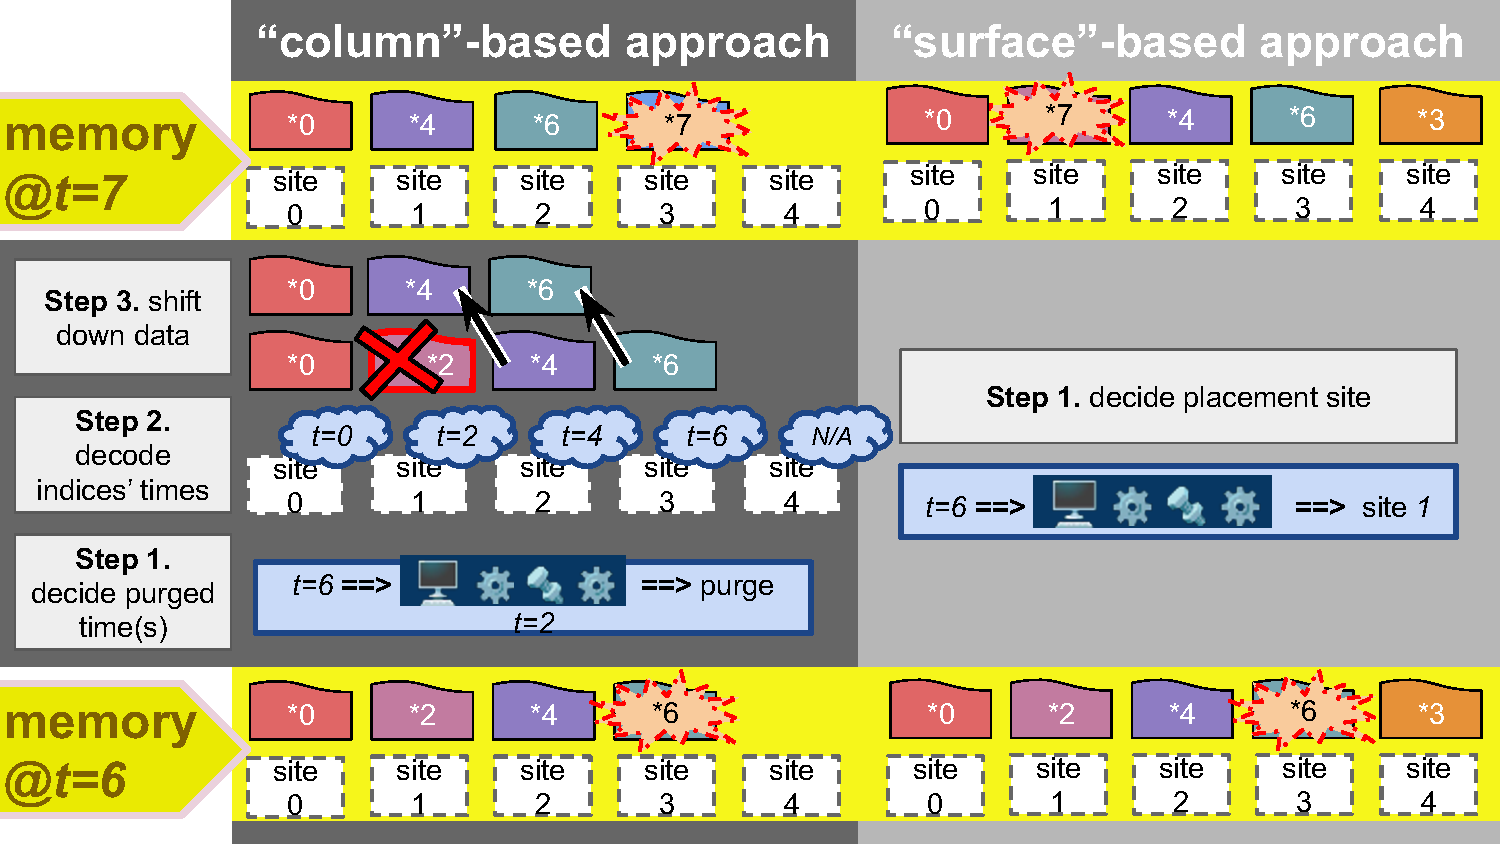
\includegraphics[width=\linewidth]{img/surf-vs-column-schematic}
  \caption{
  \textbf{Column vs. surface-based hereditary stratigraphy.}
  \footnotesize
  Contrast of existing sorted-order ``column''-based stratum retention framework with proposed explicitly addressed ``surface''-based approach.}
  \label{fig:surf-vs-column-schematic}
\end{figure}


Addressing these concerns required fundamental reformulation of hereditary stratigraphy conventions.
To this end, we introduce a constant-time indexing scheme that maps each lineage's fingerprint stream directly onto a fixed-width memory buffer.
Differentia pruning occurs implicitly, as a result of resident differentia being overwritten by new placements.
As before, care is taken to guarantee maintainance of a temporally-representative collections of resident within the memory buffer over elapsed time.
We refer to this new approach as ``surface''-based, as opposed to ``column''-based.
Figure \ref{fig:surf-vs=column-schematic} contrasts the two.
% to distinguish it from earlier conventions


% New approach uses a constant-time indexing scheme that maps each lineage's fingerprint stream onto a fixed-width memory buffer such that eviction of existing fingerprint values by new placements maintains a temporally-representative sampling over elapsed time .
% We call this approach ``surface''-based to distinguish it from earlier hereditary stratigraphy methods.
% As before, time stamps can be positionally inferred and thus do not need to be stored --- a several-fold savings that enables fingerprint values to be shrunk down and packed together.


\begin{figure*}
  \centering
\begin{subfigure}[b]{0.43\linewidth}
\centering
\textbf{steady retention policy}
\end{subfigure}
\begin{subfigure}[b]{0.43\linewidth}
\centering
\textbf{tilted retention policy}
\end{subfigure}

  \begin{subfigure}[b]{0.43\linewidth}
    \centering
  \includegraphics[height=\linewidth, angle=90,trim={0 2.4cm 0 0},clip]{binder-surface-concept/teeplots/10/cnorm=log+num-generations=4096+surface-size=256+viz=site-deposition-depth-by-rank-heatmap+ynorm=linear+ext=}
    \caption{256 bit steady surface site age plot}
    \label{fig:steady-age-plot}
  \end{subfigure}
  \begin{subfigure}[b]{0.43\linewidth}
    \centering
  \includegraphics[height=\linewidth, angle=90, trim={0 0 0 2.4cm},clip]{binder-surface-concept/teeplots/21/cnorm=log+num-generations=4096+surface-size=256+viz=site-deposition-depth-by-rank-heatmap+ynorm=linear+ext=}
    \caption{256 bit tilted surface site age plot}
    \label{fig:tilted-age-plot}
  \end{subfigure}


\begin{subfigure}[b]{0.43\linewidth}
  \flushleft
\includegraphics[height=0.7in, trim={0 0 0 0},clip]{binder-surface-concept/teeplots/10/num-generations=262144+surface-size=64+viz=stratum-persistence-dripplot+ext=}

  \centering
  \caption{64 bit steady surface time retention plot}
  \label{fig:steady-retention-plot}
\end{subfigure}
\begin{subfigure}[b]{0.43\linewidth}
  \flushright
\includegraphics[height=0.7in, trim={2.2cm 0 0 0},clip]{binder-surface-concept/teeplots/21/num-generations=262144+surface-size=64+viz=stratum-persistence-dripplot+ext=}

  \centering
  \caption{64 bit tilted surface time retention plot}
  \label{fig:tilted-retention-plot}
\end{subfigure}

\caption{%
  \textbf{Surface-based hereditary stratigraphy implementations.}
  Visualizations of steady (left) and tilted (right) surface site selection policies.
  Top row heatmaps shows evolution of time-since-last-deposition for each site on a 256 bit field over the course of 4,096 depositions.
  Bottom row shows retention spans for 3,000 ingested time points.
  Vertical lines span durations between ingestion and elimination for successive time points.
  Time points previously eliminated are marked in red.
  Note that for top row, time elapses from top to bottom and, for bottom row, time elapses bottom to top.
  }
\label{fig:surf-algorithms}

\end{figure*}


In the course of this work, steady- and tilted-policy surface-based hereditary stratigraphy algorithms have both been developed.
Figure \ref{fig:surf-algorithms} depicts implementation behaviors, with the top panels tracking how placements are sequenced over time in buffer space and the bottom panels showing the consequent distributions of retained timepoints across history.
We leave formal descriptions of underlying indexing algorithms to future work.
However, reference implementations can be found supplementary material (Listing TODO).
% For this work, we also translated the tilted algorithm to Zig--like Cerebras Software Language for use on the WSE and, as an intermediate step, to the general-purpose Zig programming language.
% These implementations can be found in associated software repositories with the project.
These algorithms are notable in providing a novel and highly-efficient solution the more general problem of curating dynamic temporal cross-samples from a data stream, and may lend themselves to a broad set of applications outside the scope of phylogeny tracking \citep{TODOCITEPREPRINT}.

% async microthread to send from sendBuf to neighbor
% fn dispatchSend_S() void {
%   @fmovs(sendDsd_S, sendBufDsd_S,
%     .{
%       .async = true,
%       .activate = sendFinalizeTaskID_S

% const recvDsd_N = @get_dsd(fabin_dsd, .{
%   .fabric_color = recvColor_N,
%   .extent = recvBufSize,
%   .input_queue = @get_input_queue(q_in_N)
% });
% // open an async microthread to recv from neighbor into recvBuf
% fn dispatchRecv_N() void {
%   @fmovs(recvBufDsd_N, recvDsd_N,
%     .{
%       .async = true,

% color swapping

\subsection{Asynchronous Island-model Genetic Algorithm}

We apply an island-model genetic algorithm to instantiate an evolutionary process spanning PEs.
Island-model approaches are common in applications of parallel and distributed computing to evolutionary computation \citep{bennett1999building}.
Under this model, each processor element (PE) hosts an independent population.
Migration between PEs stitches island populations together into a common gene pool.

Core kernel activity proceeds via an update cycle performed on each PE, which comprises several steps.
Figure \ref{fig:async-ga-schematic} provides a schematic overview.

The first step of this update loop is to handle migration, depicted as blue-red arrows in Figure \ref{fig:async-ga-schematic}.
We adopt a fully asynchronous approach to migration between neighboring PEs.
Evolutionary processes tend to occur in asynchronous manner with arbitrary factors influencing things, so this is a reasonable relaxation to make.

Each PE maintains independent immigration buffers and emigration buffers dedicated to each cardinal neighbor, depicted in blue and red, respectively, in Figure \ref{fig:async-ga-schematic}.
On simulation startup, an asynchronous DSD receive operation is opened to accept genomes from neighboring PEs into the appropriate immigration buffer.
At startup, additionally, the emigration buffer is populated with one or more genomes copied the population.
Then, an asynchronous send request is opened to dispatch wavelets containing genome data from the emigration buffer to the neighbor.
Both operations register an on-completion callback to set a ``send complete'' or ``receive complete'' flag variable associated with their corresponding buffer.

Each update cycle, the main update loop tests all ``send complete'' and ``receive complete'' flags.
For each immigration flag that is set, corresponding received genomes are written into the main population buffer, replacing randomly-chosen population members.
Then, the flag is reset a new receive request is initiated.
Likewise, for each emigration flag set, corresponding send buffers are re-populated with randomly sampled genomes from the main population buffer.
Corresponding flags are then reset and new send requests initiated.
The bottom right corner of Figure \ref{fig:async-ga-schematic} summarizes this process.

The remainder of the main update loop handles evolutionary operations within the scope of the executing PE.
Each genome within the population is evaluated to produce a floating point fitness value.
Modular implementation ensures evaluation criteria can be chosen appropriate for underlying experimental objectives.
For the purposes this project, we will use a trivial fitness function that explicitly models additive accumulation of beneficial/deleterious mutations as a floating point value within each genome.

After evaluation, tournament selection is applied.
Each slot in the next generation is populated with a genome exhibiting maximal fitness among $n$ randomly sampled individuals, ties broken randomly.

Finally, a mutational operator is applied across all genomes in the next population.
As with evaluation criteria, modular implementation allows mutation operations to be defined based on experimental objectives.
Here, we use a simple Gaussian mutation on each genome's stored fitness value.
At this point, hereditary stratigraphy annotations --- discussed next --- are updated to reflect an elapsed generation.

The process then repeats, with self-activating wavelet dispatched to execute the next cycle of the main update loop.

% Define lighter colors
\definecolor{LighterBlue}{rgb}{0.84, 0.92, 0.95}
\definecolor{LighterSalmon}{rgb}{1.0, 0.81, 0.76}
\definecolor{LighterPastelGreenYellow}{rgb}{0.88, 0.96, 0.90}

% Define thick vertical lines for section dividers
\newcolumntype{q}{!{\color{white} \vrule width 2pt}}

\begin{figure*}
    \centering
\begin{tabular}{
c
>{\columncolor{LighterBlue}}c
>{\columncolor{LighterBlue}}c
>{\columncolor{LighterSalmon}}c
>{\columncolor{LighterSalmon}}c
q % Thick divider
>{\columncolor{LighterPastelGreenYellow}}c
>{\columncolor{LighterPastelGreenYellow}}c
>{\columncolor{LighterPastelGreenYellow}}c
>{\columncolor{LighterPastelGreenYellow}}c
q % Thick divider
>{\columncolor{LighterPastelGreenYellow}}c
>{\columncolor{LighterPastelGreenYellow}}c
>{\columncolor{LighterPastelGreenYellow}}c
>{\columncolor{LighterPastelGreenYellow}}c
}
& \multicolumn{4}{cq}{\cellcolor{white}Word 0} & \multicolumn{4}{cq}{\cellcolor{white}Word 1} & \multicolumn{4}{c}{\cellcolor{white}Word 2} \\
\cmidrule(l{1.5pt}r{1.5pt}){2-5}
\cmidrule(l{1.5pt}r{1.5pt}){6-9}
\cmidrule(l{1.5pt}r{1.5pt}){10-13}
Byte & {\cellcolor{white}0} & {\cellcolor{white}1} & {\cellcolor{white}2} & {\cellcolor{white}3} & {\cellcolor{white}4} & {\cellcolor{white}5} & {\cellcolor{white}6} & {\cellcolor{white}7} & {\cellcolor{white}8} & {\cellcolor{white}9} & {\cellcolor{white}10} & {\cellcolor{white}11} \\
\cmidrule(l{1.5pt}r{1.5pt}){2-2}
\cmidrule(l{1.5pt}r{1.5pt}){3-3}
\cmidrule(l{1.5pt}r{1.5pt}){4-4}
\cmidrule(l{1.5pt}r{1.5pt}){5-5}
\cmidrule(l{1.5pt}r{1.5pt}){6-6}
\cmidrule(l{1.5pt}r{1.5pt}){7-7}
\cmidrule(l{1.5pt}r{1.5pt}){8-8}
\cmidrule(l{1.5pt}r{1.5pt}){9-9}
\cmidrule(l{1.5pt}r{1.5pt}){10-10}
\cmidrule(l{1.5pt}r{1.5pt}){11-11}
\cmidrule(l{1.5pt}r{1.5pt}){12-12}
\cmidrule(l{1.5pt}r{1.5pt}){13-13}
& \multicolumn{4}{cq}{\cellcolor{white}} & \multicolumn{4}{cq}{\cellcolor{white}} & \multicolumn{4}{c}{\cellcolor{white}} \\[-2ex]
Genome 0 & \texttt{F9} & \texttt{02} & \texttt{79} & \texttt{00} & \texttt{8D} & \texttt{22} & \texttt{4F} & \texttt{F3} & \texttt{D2} & \texttt{78} & \texttt{AD} & \texttt{C7} \\
& \multicolumn{4}{cq}{\cellcolor{white}} & \multicolumn{4}{cq}{\cellcolor{white}} & \multicolumn{4}{c}{\cellcolor{white}} \\[-2ex]
Genome 1 & \texttt{F9} & \texttt{02} & \texttt{75} & \texttt{00} & \texttt{8D} & \texttt{A1} & \texttt{CB} & \texttt{F2} & \texttt{D1} & \texttt{5B} & \texttt{CC} & \texttt{D4} \\
& \multicolumn{4}{cq}{\cellcolor{white}} & \multicolumn{4}{cq}{\cellcolor{white}} & \multicolumn{4}{c}{\cellcolor{white}} \\[-2ex]
Genome 2 & \texttt{61} & \texttt{B6} & \texttt{65} & \texttt{00} & \texttt{66} & \texttt{29} & \texttt{B4} & \texttt{F0} & \texttt{62} & \texttt{99} & \texttt{5A} & \texttt{61} \\
{\cellcolor{white}\ldots} & {\cellcolor{white}\ldots} & {\cellcolor{white}\ldots} & {\cellcolor{white}\ldots} & {\cellcolor{white}\ldots} & {\cellcolor{white}\ldots} & {\cellcolor{white}\ldots} & {\cellcolor{white}\ldots} & {\cellcolor{white}\ldots} & {\cellcolor{white}\ldots} & {\cellcolor{white}\ldots} &
{\cellcolor{white}\ldots} & {\cellcolor{white}\ldots} \\
\end{tabular}

\caption{%
\textbf{Example genomes sampled after simulation completion.}
  In validation testing, genomes were composed of three 32-bit words.
  The first two bytes (blue) are fixed random markers generated at simulation start-up, indicating independent lineage originations.
  The next two bytes (salmon) are a generation counter.
  Bits within the final eight bytes are lineage checkpoint values to facilitate phylogenetic reconstruction, arranged according to a tilted hereditary stratigraphic algorithm.
  Note that this genome does not include any content affecting agent traits or fitness --- neutral selection was used for this validation experiment.
}
\label{fig:genome-layout}
\end{figure*}


Kernel source code implementing described procedures can be viewed at \url{https://hopth.ru/cl}.
Our implementation is defined modularity with respect to genome size, layout, mutational operator, and fitness evaluation criteria, allowing for direct re-use of produced software for follow-on evolution experiments on WSE hardware.
Figure \ref{fig:genome-layout} shows an example genome layout including hstrat instrumentation.


In preparation for proposed work, we joined the Cerebras SDK program \citep{selig2022cerebras} and assembled Cerebras Software Language (CSL) software implementations that will be necessary to conduct experiments with WSE hardware.
For the time being, we have used Cerebras' hardware emulator to test our software implementations.
This section reports a small-scale experiment performed to validate the core software functionality.
In addition to this integration test, software quality has also been verified through an associated unit test suite.

Genomes were fixed-length 3 word arrays represented using data type \texttt{u32}.
Figure \ref{fig:validation-example:genomes} details the content and layout of genomes, and provides example genome values yielded from simulation.
Notably, the first sixteen bits were used to tag clade geneses.
At the outset of simulation, founding population members were each assigned a randomized tag value.
This value was inherited without mutation over the course of simulation.
Thus, it can be used to identify end-state genomes that evolved from the same original ancestor.

The send buffers were sized to hold one genome and the receive buffers to hold 4 genomes.

% A key question will be the extent to which intentionally desynchronizing affects performance, stability, and computation quality.

\subsection{Software and Data Availability}

Software, configuration files, and executable notebooks for this work are available at \url{https://github.com/mmore500/hstrat-wafer-scale} TODO.
CSL Software can be found on at \url{https://github.com/mmore500/wse-sketches/tree/v0.1.0} \citep{moreno2024wse}.
Data and supplemental materials are available via the Open Science Framework \url{https://osf.io/bfm2z/} \citep{foster2017open}.

All hereditary stratigraph annotation, reference phylogeny generation, and phylogenetic reconstruction tools used in this work are published in the \texttt{hstrat} Python package \citep{moreno2022hstrat}.
This project uses data formats and tools associated with the ALife Data Standards project \citep{lalejini2019data} and benefited from many pieces of open-source scientific software \citep{sand2014tqdist,2020SciPy-NMeth,harris2020array,reback2020pandas,mckinney-proc-scipy-2010,sukumaran2010dendropy,cock2009biopython,dolson2024phylotrackpy,torchiano2016effsize,waskom2021seaborn,hunter2007matplotlib,moreno2024apc,moreno2023teeplot,torchiano2016effsize,moreno2024pecking,moreno2024joinem,moreno2024hsurf}.

The experiments in this use the Cerebras SDK to compile and test on a hardware simulator \citep{TODOCITE}.
Access to the SDK can be requested, currently free of charge, via their website.
